% unit: u12
% sources: sources/070-matrix-spaces-rank-1-small-world-graphs.txt, sources/162-matrix-spaces-rank-1-small-world-graphs.txt, sources/163-mit18-06scf11-ses1-11sum-pdf-download-file.txt, sources/164-matrix-spaces.txt, sources/165-mit18-06scf11-ses1-11prob-pdf-download-file.txt, sources/166-mit18-06scf11-ses1-11sol-pdf-download-file.txt
\section{Matrix spaces; rank one; small world graphs}\label{sec:u12}

Everything in Sections~\ref{sec:u10} and~\ref{sec:u11} used only two operations: adding vectors and
multiplying them by numbers. So the same ideas (subspace, basis, dimension) apply to any objects
that can be added and scaled. This section works them out for spaces of matrices and a space of
functions, introduces two natural operations on subspaces (intersection and sum), shows that
rank-one matrices are the building blocks of every matrix, and ends with the graphs that lead into
Section~\ref{sec:u13}.

\subsection{Bases and dimensions of matrix spaces}

Let $M$ be the space of all $3\times3$ matrices (Example~\ref{ex:u11-M}). Write $E_{ij}$ for the
matrix with a $1$ in position $(i,j)$ and zeros elsewhere.

\begin{proposition}[Dimensions in \texorpdfstring{\(M\)}{M}]\label{prop:u12-dims}
\begin{enumerate}[(a)]
\item The nine matrices $E_{ij}$ form a basis of $M$, so $\dim M=9$.
\item The six $E_{ij}$ with $i\le j$ form a basis of the upper triangular matrices $U$: $\dim U=6$.
\item $E_{11},E_{22},E_{33},\ E_{12}+E_{21},\ E_{13}+E_{31},\ E_{23}+E_{32}$ form a basis of the
symmetric matrices $S$: $\dim S=6$.
\item $E_{11},E_{22},E_{33}$ form a basis of the diagonal matrices $D=S\cap U$: $\dim D=3$.
\end{enumerate}
\end{proposition}
\begin{proof}
(a) $A=\sum_{i,j}a_{ij}E_{ij}$, and this combination is the zero matrix only if every $a_{ij}=0$.
(b) The same argument applies to matrices with $a_{ij}=0$ for $i>j$. (c) A symmetric matrix is
determined by its three diagonal entries and three entries above the diagonal:
$A=\sum_i a_{ii}E_{ii}+\sum_{i<j}a_{ij}(E_{ij}+E_{ji})$, and the six coefficients are entries of
$A$, so the combination vanishes only when they are all $0$. (d) As in (a).
\end{proof}

So $M$ is ``practically $\R^9$'', with the nine numbers written in a square. The bases of $U$ and
$D$ happen to be subsets of the standard basis of $M$; the basis of $S$ cannot be, because only three
of the nine $E_{ij}$ are symmetric. In general a subspace needs its own basis.

\subsection{Intersections and sums of subspaces}

\begin{proposition}[Intersection]\label{prop:u12-cap}
If $V$ and $W$ are subspaces of the same space, so is $V\cap W$.
\end{proposition}
\begin{proof}
If $\vb{x},\vb{y}$ lie in both $V$ and $W$, then $\vb{x}+\vb{y}$ and $c\vb{x}$ lie in $V$ (a
subspace) and in $W$ (a subspace).
\end{proof}

The union $V\cup W$ is usually \emph{not} a subspace: two different lines through the origin in
$\R^2$ are not closed under addition (Figure~\ref{fig:u12-sum}). To get a subspace we must fill in
between them.

\begin{definition}[Sum of subspaces]\label{def:u12-sum}
The \emph{sum} of subspaces $V$ and $W$ is $V+W=\{\vb{v}+\vb{w}:\vb{v}\in V,\ \vb{w}\in W\}$.
\end{definition}

$V+W$ is a subspace: $(\vb{v}+\vb{w})+(\vb{v}'+\vb{w}')=(\vb{v}+\vb{v}')+(\vb{w}+\vb{w}')$ and
$c(\vb{v}+\vb{w})=c\vb{v}+c\vb{w}$. It is the smallest subspace containing $V\cup W$, since any
subspace containing both must contain all such sums.

\begin{figure}[ht]\centering
\begin{tikzpicture}[scale=0.85,>=Stealth,font=\small]
  \fill[blue!5] (-2.6,-1.4) rectangle (3.4,2.9);
  \draw[->,gray] (-2.6,0) -- (3.4,0);
  \draw[->,gray] (0,-1.4) -- (0,2.9);
  \draw[very thick,blue!70!black] (-2.6,-0.78) -- (3.4,1.02) node[below left] {$V$};
  \draw[very thick,orange!80!black] (-0.7,-1.4) -- (1.45,2.9) node[below right] {$W$};
  \draw[->,thick,blue!70!black] (0,0) -- (2,0.6) node[below right=-1pt] {$\vb{v}$};
  \draw[->,thick,orange!80!black] (0,0) -- (0.65,1.3) node[left] {$\vb{w}$};
  \draw[dashed] (2,0.6) -- (2.65,1.9) -- (0.65,1.3);
  \draw[->,very thick] (0,0) -- (2.65,1.9) node[above right] {$\vb{v}+\vb{w}$};
  \node[anchor=south east,align=right,font=\footnotesize] at (3.35,-1.35) {$V+W=\R^2$ (shaded)};
\end{tikzpicture}
\caption{Two lines $V$ and $W$ through the origin. Their union is not a subspace: $\vb{v}+\vb{w}$
lies on neither line. Their sum $V+W$ is the whole plane, and their intersection is $\{\vb{0}\}$,
so $\dim(V+W)+\dim(V\cap W)=2+0=1+1$.}
\label{fig:u12-sum}
\end{figure}

\begin{example}[Symmetric plus upper triangular]\label{ex:u12-SU}
$S+U=M$: every $3\times3$ matrix is a symmetric matrix plus an upper triangular one. Copy the part
below the diagonal into a symmetric matrix and put the rest into the upper triangular one:
\[
\begin{bmatrix}1&2&3\\4&5&6\\7&8&9\end{bmatrix}
=\begin{bmatrix}0&4&7\\4&0&8\\7&8&0\end{bmatrix}
+\begin{bmatrix}1&-2&-4\\0&5&-2\\0&0&9\end{bmatrix}.
\]
The same recipe works for every matrix. Note the dimensions: $\dim S+\dim U=6+6$ and
$\dim(S+U)+\dim(S\cap U)=9+3$.
\end{example}

\begin{theorem}[Dimension of a sum]\label{thm:u12-sumdim}
For finite-dimensional subspaces $V$ and $W$ of the same space,
\[
\dim(V+W)+\dim(V\cap W)=\dim V+\dim W.
\]
\end{theorem}
\begin{proof}
Let $\vb{u}_1,\dots,\vb{u}_k$ be a basis of $V\cap W$. By Proposition~\ref{prop:u10-right}(c)
it extends to a basis of $V$, say $\vb{u}_1,\dots,\vb{u}_k$, $\vb{v}_1,\dots,\vb{v}_p$, and to a
basis of $W$, say $\vb{u}_1,\dots,\vb{u}_k$, $\vb{w}_1,\dots,\vb{w}_q$. We claim that all $k+p+q$
vectors $\vb{u}_i,\vb{v}_j,\vb{w}_l$ together form a basis of $V+W$; then
$\dim(V+W)+\dim(V\cap W)=(k+p+q)+k=(k+p)+(k+q)$, as required.

They span $V+W$, since every $\vb{v}\in V$ and every $\vb{w}\in W$ is a combination of them. For
independence, suppose $\sum a_i\vb{u}_i+\sum b_j\vb{v}_j+\sum c_l\vb{w}_l=\vb{0}$. Then
$\vb{z}=\sum c_l\vb{w}_l=-\sum a_i\vb{u}_i-\sum b_j\vb{v}_j$ lies in $W$ (left side) and in $V$
(right side), hence in $V\cap W$, so $\vb{z}=\sum d_i\vb{u}_i$ for some $d_i$. Then
$\sum c_l\vb{w}_l-\sum d_i\vb{u}_i=\vb{0}$, and independence of the basis of $W$ gives all
$c_l=0$ (and $d_i=0$). Now $\sum a_i\vb{u}_i+\sum b_j\vb{v}_j=\vb{0}$, and independence of the
basis of $V$ gives all $a_i=b_j=0$.
\end{proof}

\begin{trap}
The dimension formula involves the \emph{sum} $V+W$, not the union. ``$\dim(S\cup U)$'' has no
meaning, because $S\cup U$ is not a vector space: the symmetric matrix $E_{12}+E_{21}$ plus the
upper triangular matrix $E_{12}$ is $2E_{12}+E_{21}$, which is neither symmetric nor upper
triangular.
\end{trap}

\subsection{A space of functions}

The solutions of the differential equation
\[
\frac{d^2y}{dx^2}+y=0
\]
form a vector space: if $y_1''+y_1=0$ and $y_2''+y_2=0$ then $(c_1y_1+c_2y_2)''+(c_1y_1+c_2y_2)=0$.
It is the ``nullspace'' of the operation $y\mapsto y''+y$. Both $\cos x$ and $\sin x$ are in it.

\begin{theorem}[Solutions of \texorpdfstring{\(y''+y=0\)}{y''+y=0}]\label{thm:u12-ode}
$\cos x$ and $\sin x$ form a basis of the solution space, which therefore has dimension $2$. The
solution with $y(0)=a$ and $y'(0)=b$ is $y=a\cos x+b\sin x$.
\end{theorem}
\begin{proof}
\emph{Independent:} if $c_1\cos x+c_2\sin x=0$ for all $x$, then $x=0$ gives $c_1=0$ and
$x=\pi/2$ gives $c_2=0$.
\emph{Spanning:} let $y$ be any solution and put $z=y-y(0)\cos x-y'(0)\sin x$. Then $z$ is a
solution with $z(0)=0$ and $z'(0)=0$. The quantity $E=z^2+(z')^2$ satisfies
$E'=2zz'+2z'z''=2z'(z+z'')=0$, so $E$ is constant, equal to $E(0)=0$. Hence $z\equiv0$ and
$y=y(0)\cos x+y'(0)\sin x$.
\end{proof}

These two functions play the role of the special solutions: a second-order equation has a
two-dimensional solution space, and solving it means finding a basis. Other bases exist; if complex
scalars are allowed, $e^{ix}$ and $e^{-ix}$ form one (they are $\cos x\pm i\sin x$). For example,
the solution with $y(0)=2$ and $y'(0)=-1$ is $y=2\cos x-\sin x$; check:
$y''=-2\cos x+\sin x=-y$.

\subsection{Rank-one matrices}

\begin{example}[A column times a row]\label{ex:u12-rank1}
In $A=\begin{bmatrix}1&4&5\\2&8&10\end{bmatrix}$ the second row is twice the first, so the rank is
$1$. A basis of the row space is $(1,4,5)$, a basis of the column space is $(1,2)$, and every column
is a multiple of $(1,2)$, with multipliers $1,4,5$. That is exactly the product
\[
A=\begin{bmatrix}1\\2\end{bmatrix}\begin{bmatrix}1&4&5\end{bmatrix}.
\]
\end{example}

\begin{theorem}[Rank one]\label{thm:u12-rank1}
A matrix has rank $1$ if and only if it equals $\vb{u}\vb{v}\T$ for some nonzero column vectors
$\vb{u}\in\R^m$, $\vb{v}\in\R^n$. Then $\Col{A}$ is the line through $\vb{u}$, $\Col{A\T}$ is the
line through $\vb{v}$, and $\Nul{A}=\{\vb{x}:\vb{v}\T\vb{x}=0\}$.
\end{theorem}
\begin{proof}
Column $j$ of $\vb{u}\vb{v}\T$ is $v_j\vb{u}$, so every column lies on the line through $\vb{u}$,
and some column is nonzero because $\vb{v}\ne\vb{0}$ and $\vb{u}\ne\vb{0}$; hence the column space
is that line and the rank is $1$. Conversely, if $\rank A=1$, then $\Col{A}$ has a basis consisting
of one vector $\vb{u}$, so each column is $\vb{a}_j=v_j\vb{u}$ for some number $v_j$; that says
$A=\vb{u}\vb{v}\T$, and $\vb{v}\ne\vb{0}$ because $A\ne0$. The same argument applied to the rows
($A\T=\vb{v}\vb{u}\T$) gives the row space. Finally
$A\vb{x}=\vb{u}(\vb{v}\T\vb{x})=\vb{0}$ exactly when the number $\vb{v}\T\vb{x}$ is $0$.
\end{proof}

\begin{example}[The four subspaces of \texorpdfstring{\(\begin{bmatrix}1&1&1&1\end{bmatrix}\)}{[1 1 1 1]}]\label{ex:u12-sum0}
The vectors $\vb{v}\in\R^4$ with $v_1+v_2+v_3+v_4=0$ form a subspace, the nullspace of the
rank-one matrix $A=\begin{bmatrix}1&1&1&1\end{bmatrix}$ ($m=1$, $n=4$, $r=1$). The pivot variable
is $v_1$, and the three special solutions
\[
(-1,1,0,0),\qquad(-1,0,1,0),\qquad(-1,0,0,1)
\]
are a basis, so the dimension is $n-r=3$. The row space is the line through $(1,1,1,1)$
(dimension~1); $3+1=4$. The column space is all of $\R^1$ (dimension $1$), and the left nullspace is
$\{0\}$ (dimension $0$, with the empty set as basis); $1+0=1$.
\end{example}

Rank-one matrices are the building blocks of all matrices.

\begin{theorem}[A sum of rank-one pieces]\label{thm:u12-CR}
Let $A$ have rank $r$, let $C$ be the $m\times r$ matrix of pivot columns of $A$, and let $R_0$ be
the $r\times n$ matrix of nonzero rows of $R=\operatorname{rref}(A)$. Then $A=CR_0$; equivalently, $A$
is the sum of the $r$ rank-one matrices $(\text{pivot column }k)(\text{row }k\text{ of }R_0)$.
\end{theorem}
\begin{proof}
Column $j$ of $CR_0$ is $C$ times column $j$ of $R_0$. If $j$ is the $k$th pivot column, column $j$
of $R_0$ is the $k$th standard basis vector and the product is the $k$th column of $C$, which is
$\vb{a}_j$. If $j$ is free, column $j$ of $R_0$ holds the entries $f_{1j},\dots,f_{rj}$ of $F$ in
that column, and the special solution $\vb{s}_j$ (pivot entries $-f_{kj}$, entry $1$ in position $j$)
gives $A\vb{s}_j=\vb{a}_j-\sum_kf_{kj}(\text{pivot column }k)=\vb{0}$. So
$\vb{a}_j=\sum_kf_{kj}(\text{pivot column }k)$, which is again column $j$ of $CR_0$. The column-row
expansion of a product then writes $CR_0$ as a sum of $r$ column-times-row terms.
\end{proof}

For the matrix of Example~\ref{ex:u11-four} this reads
\[
\begin{bmatrix}1&2&3&1\\1&1&2&1\\1&2&3&1\end{bmatrix}
=\begin{bmatrix}1\\1\\1\end{bmatrix}\begin{bmatrix}1&0&1&1\end{bmatrix}
+\begin{bmatrix}2\\1\\2\end{bmatrix}\begin{bmatrix}0&1&1&0\end{bmatrix},
\]
two rank-one pieces for a rank-two matrix. In the same way a $5\times17$ matrix of rank $4$ is a sum
of four rank-one matrices.

\begin{proposition}[Rank of a sum]\label{prop:u12-subadd}
$\rank(A+B)\le\rank A+\rank B$ for matrices of the same size.
\end{proposition}
\begin{proof}
Every column of $A+B$ is a column of $A$ plus a column of $B$, so $\Col{A+B}\subseteq\Col{A}+\Col{B}$.
By Theorem~\ref{thm:u12-sumdim}, $\dim(\Col{A}+\Col{B})\le\dim\Col{A}+\dim\Col{B}$.
\end{proof}

Consequently the rank-one matrices do \emph{not} form a subspace of $M$: $E_{11}+E_{22}$ has rank $2$.
Nor do the $5\times17$ matrices of rank at most $4$ (even with the zero matrix included): with
$E_{ij}$ now $5\times17$, the matrices $E_{11}+E_{22}+E_{33}+E_{44}$ and
$E_{22}+E_{33}+E_{44}+E_{55}$ have rank $4$, but their sum has the five pivots $1,2,2,2,1$ and rank
$5$.

\subsection{Small world graphs}

\begin{definition}[Graph, distance, diameter]\label{def:u12-graph}
A \emph{graph} $G=\{\text{nodes},\text{edges}\}$ is a set of nodes together with edges, each edge
joining two nodes. The \emph{distance} between two nodes is the smallest number of edges in a path
joining them; the \emph{diameter} is the largest distance between two nodes.
\end{definition}

Take one node for each person in a country and an edge between any two people who are friends. The
phrase ``six degrees of separation'' is the claim that this graph has small diameter, roughly six;
when two strangers on a plane find a mutual friend they remark that it is a small world. The World
Wide Web, with sites as nodes and links as edges, raises the same question. The mathematical point
is that a few long-range shortcuts make all distances drop dramatically.

\begin{example}[A ring with shortcuts]\label{ex:u12-ring}
Put $12$ people in a ring, each friends only with the two neighbours. The distance between nodes
$i$ and $j$ is $\min(|i-j|,\,12-|i-j|)$, so the diameter is $6$. From any node the other eleven are
at distances $1,1,2,2,3,3,4,4,5,5,6$, which sum to $36$: the average distance is
$36/11\approx3.27$. Now add the long-range friendships $1$--$7$, $3$--$9$, $5$--$11$ one at a time
(Figure~\ref{fig:u12-ring}). Breadth-first search from every node gives
\begin{center}
\begin{tabular}{@{}lcccc@{}}
\toprule
shortcuts added & none & $1$--$7$ & $+\ 3$--$9$ & $+\ 5$--$11$\\
\midrule
diameter & $6$ & $6$ & $5$ & $3$\\
average distance & $3.27$ & $2.74$ & $2.39$ & $2.18$\\
\bottomrule
\end{tabular}
\end{center}
Three extra edges out of fifteen halve the diameter. For instance, after all three shortcuts node
$2$ reaches node $8$ in three steps ($2\to1\to7\to8$) instead of six.
\end{example}

\begin{figure}[ht]\centering
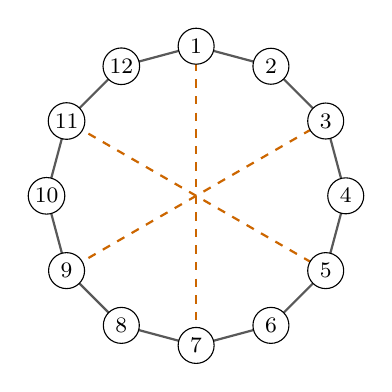
\begin{tikzpicture}[font=\footnotesize]
  \foreach \k in {1,...,12} {
    \coordinate (n\k) at ({90-30*(\k-1)}:1.9);
  }
  \foreach \k [evaluate=\k as \nxt using {int(mod(\k,12)+1)}] in {1,...,12} {
    \draw[thick,gray!70!black] (n\k) -- (n\nxt);
  }
  \draw[thick,dashed,orange!80!black] (n1) -- (n7);
  \draw[thick,dashed,orange!80!black] (n3) -- (n9);
  \draw[thick,dashed,orange!80!black] (n5) -- (n11);
  \foreach \k in {1,...,12} {
    \node[circle,draw,fill=white,inner sep=1.2pt,minimum size=13pt] at (n\k) {\k};
  }
\end{tikzpicture}
\caption{A ring of $12$ friends (solid) with three long-range shortcuts (dashed). Without shortcuts
the diameter is $6$; with them it is $3$.}
\label{fig:u12-ring}
\end{figure}

To study such questions with linear algebra we need a matrix for every graph. Section~\ref{sec:u13}
builds it, the incidence matrix, for a small directed graph.

\subsection{Exercises}

\begin{exercise}\label{exr:u12-perm}
Write the $3\times3$ identity as a combination of the other five $3\times3$ permutation matrices,
and show that those five are linearly independent. (They form a basis of the subspace of
$3\times3$ matrices whose row and column sums are all equal.)
\end{exercise}
\begin{solution}
The other five are $P_{21},P_{31},P_{32}$ (exchanging two rows of $I$) and the cyclic shifts
\[
P_{32}P_{21}=\begin{bmatrix}0&1&0\\0&0&1\\1&0&0\end{bmatrix},\qquad
P_{21}P_{32}=\begin{bmatrix}0&0&1\\1&0&0\\0&1&0\end{bmatrix}.
\]
$P_{21}+P_{31}+P_{32}$ is the all-ones matrix and $P_{32}P_{21}+P_{21}P_{32}$ has zeros on the diagonal
and ones elsewhere, so $I=P_{21}+P_{31}+P_{32}-P_{32}P_{21}-P_{21}P_{32}$. For independence,
\[
c_1P_{21}+c_2P_{31}+c_3P_{32}+c_4P_{32}P_{21}+c_5P_{21}P_{32}=
\begin{bmatrix}c_3&c_1+c_4&c_2+c_5\\c_1+c_5&c_2&c_3+c_4\\c_2+c_4&c_3+c_5&c_1\end{bmatrix}.
\]
If this is zero, the diagonal gives $c_1=c_2=c_3=0$ and then the off-diagonal entries give
$c_4=c_5=0$.
\end{solution}

\begin{exercise}\label{exr:u12-AX}
Let $M$ be the space of $3\times3$ matrices and $A=\begin{bmatrix}1&0&-1\\-1&1&0\\0&-1&1\end{bmatrix}$.
Consider the operation $X\mapsto AX$ on $M$. (a) Which $X$ give $AX=0$? (b) Which matrices have
the form $AX$? (c) What are the dimensions of these two subspaces of $M$, and why do they add to $9$?
\end{exercise}
\begin{solution}
(a) $A$ has rank $2$ (the rows add to zero, and the first two are independent), and
$\Nul{A}$ is the line through $(1,1,1)$. $AX=0$ means every column of $X$ lies in $\Nul{A}$, so
$X=\begin{bmatrix}a&b&c\\a&b&c\\a&b&c\end{bmatrix}$. (b) The columns of $AX$ are combinations of the
columns of $A$, all of which have components summing to $0$; and since $\Col{A}$ is the whole
plane of such vectors (dimension $2$), every matrix whose columns each sum to $0$ is some $AX$.
(c) The ``nullspace'' has dimension $3$ ($a,b,c$ free) and the ``column space'' has dimension $6$
(each of three columns lies in a $2$-dimensional plane). $3+6=9=\dim M$: the count
$(n-r)+r=n$ for an operation on a $9$-dimensional input space, column by column $1+2=3$.
\end{solution}

\begin{exercise}\label{exr:u12-211}
Show that the $2\times3$ matrices $A$ with $(2,1,1)$ in their nullspace form a subspace of the
space of $2\times3$ matrices, and find a basis and its dimension. Do the $2\times3$ matrices whose
column space contains $(2,1)$ form a subspace?
\end{exercise}
\begin{solution}
If $A(2,1,1)=\vb{0}$ and $B(2,1,1)=\vb{0}$ then $(A+B)(2,1,1)=\vb{0}$ and $(cA)(2,1,1)=\vb{0}$, so it
is a subspace. Each row $(a,b,c)$ must satisfy $2a+b+c=0$, i.e.\ $c=-2a-b$, so each row is a
combination of $(1,0,-2)$ and $(0,1,-1)$. A basis is
\[
\begin{bmatrix}1&0&-2\\0&0&0\end{bmatrix},\
\begin{bmatrix}0&1&-1\\0&0&0\end{bmatrix},\
\begin{bmatrix}0&0&0\\1&0&-2\end{bmatrix},\
\begin{bmatrix}0&0&0\\0&1&-1\end{bmatrix},
\]
and the dimension is $4$. The second set is not a subspace: the zero matrix has column space
$\{\vb{0}\}$, which does not contain $(2,1)$, yet every subspace contains the zero vector.
\end{solution}

\begin{exercise}\label{exr:u12-uvT}
Write $A=\begin{bmatrix}2&-4&6\\-1&2&-3\\3&-6&9\end{bmatrix}$ as $\vb{u}\vb{v}\T$, and give a basis
for each of its four subspaces.
\end{exercise}
\begin{solution}
Every row is a multiple of $(1,-2,3)$, with multipliers $2,-1,3$, so
$A=\vb{u}\vb{v}\T$ with $\vb{u}=(2,-1,3)$ and $\vb{v}=(1,-2,3)$, and $r=1$. By
Theorem~\ref{thm:u12-rank1}: $\Col{A}$ has basis $(2,-1,3)$; $\Col{A\T}$ has basis $(1,-2,3)$;
$\Nul{A}$ is the plane $x_1-2x_2+3x_3=0$, with special solutions $(2,1,0)$ and $(-3,0,1)$; and
$\Nul{A\T}$ is the plane $2y_1-y_2+3y_3=0$, with special solutions $(\tfrac12,1,0)$ and
$(-\tfrac32,0,1)$. Dimensions $1,2,1,2$, consistent with $r=1$, $n-r=2$, $m-r=2$.
\end{solution}
